
% Beamer document class
\documentclass[xcolor=dvipsnames]{beamer}
% packages
\usepackage[utf8]{inputenc}
%\usepackage{latexsym}
\usepackage{graphicx}
\usepackage{mathptmx}
\usepackage{amsmath}
\usepackage{amsfonts}
\usepackage{amssymb}
\usepackage{amsbsy}
\usepackage{amsthm}
\usepackage{algorithmic}

% Get checkmark logo
\usepackage{pifont}
\newcommand{\cmark}{\ding{51}}
\newcommand{\xmark}{\ding{55}}

% \lee and \gee symbol
\def\lee{\mathrel{\vcenter{\hbox{$\scriptstyle\mathord<$}\nointerlineskip
\vskip 1pt\hbox{$\scriptstyle\mathord=$}}}}
\def\gee{\mathrel{\vcenter{\hbox{$\scriptstyle\mathord>$}\nointerlineskip
\vskip 1pt\hbox{$\scriptstyle\mathord=$}}}}

% Set VT theme
\usepackage{pgf} % For image/line placement.
% Set a minimal theme with maroon background colors
\setbeamercolor*{palette tertiary}{bg=Maroon}
\setbeamercolor{frametitle}{fg=Black}
\setbeamercolor{section in toc}{fg=Black}
\setbeamercolor{subsection in toc}{fg=Black}
\setbeamercolor{title}{fg=Black}
\setbeamercolor{item}{fg=Black}
\setbeamercolor{block title}{fg=Black,bg=Maroon!20}
\setbeamercolor{caption name}{fg=Black}
% Set the math fonts
\usefonttheme[onlymath]{serif}
\DeclareMathAlphabet{\mathcal}{OMS}{cmsy}{m}{n}
% Create a maroon hline under the frame title
\newcommand{\VThline}{%
\raisebox{-12mm}[0pt][0pt]{%
\begin{pgfpicture}{0mm}{0mm}{0mm}{0mm}
\pgfsetlinewidth{0.28mm}
\color{Maroon}
\pgfline{\pgfpoint{-3mm}{1mm}}{\pgfpoint{10.8cm}{1mm}}
\end{pgfpicture}}}
\setbeamertemplate{headline}{\VThline}
% Add the VT logo to the top right
\newcommand{\VTlogo}{
\vspace*{0.4cm}\hspace*{-3cm}
{
\includegraphics[height=0.5cm]{VPIlogo.png}}}
\setbeamertemplate{sidebar canvas right}{\VTlogo}
% Add page numbers
\setbeamertemplate{footline}[frame number]

% Title Information
\title{Mathematical Software for Multiobjective Optimization Problems}
\subtitle{{\bf Final Examination of Tyler H. Chang}\\
\medskip
In partial fulfillment of the requirements for the degree of\\
Ph.D. in Computer Science}
\author{Readers:\\
L.T.~Watson (chair), C.~Beattie, A.R.~Butt,\\
S.~Raghvendra, and M.W.~Trosset}
\date{May 13, 2020}
\institute{Virginia Polytechnic Institute and State University}

\begin{document}
% Make title frame with footnote
\begin{frame}[plain] % plain removes the formatting
\vfill
\titlepage
\vfil % No skip above the logo. If logo is removed, change to \vfill
% Adds logo to bottom of the title page
\centerline{
\includegraphics[height=0.5cm]{VPIlogo.png}}
\end{frame}

\section{Introduction}
% High-level MOP defn
\begin{frame}{Two Related Problems}
\begin{enumerate}
\item The multiobjective optimization problem (MOP) attempts to balance the
tradeoff between multiple conflicting objectives
\begin{itemize}
\item Objectives are conflicting, so there is no ``ideal solution''
\item Find many (approximate) solutions along the tradeoff curve and defer
to the decision maker
\item Examples: aircraft engineering, portfolio allocation, computational
chemistry, model fitting/control theory
\end{itemize}
\pause
\item The multivariate interpolation problem (MIP) predicts the outcome of an
event based on a database of past observations
\begin{itemize}
\item Must exactly match all observations in the database
\item Appropriate when predictions are deterministic in nature
\item Related to MOP, e.g., response surface modeling
\item Other examples: science/engineering models, machine learning, data science
\end{itemize}
\end{enumerate}
\end{frame}

% Make ToC
\begin{frame}{Table of Contents}
\tableofcontents
\end{frame}

% Symbols/terminology
\begin{frame}{Nomenclature}
\begin{itemize}
\item Predict/optimize the function $F : \mathbb{R}^d\rightarrow\mathbb{R}^p$
\item $x,y,z$ will denote arbitrary points in $\mathbb{R}^d$;
\item For real $n$-tuples $u,v$:
\begin{itemize}
\item $u < v$ if $u$ is componentwise strictly less than $v$;
\item $u \lee v$ if $u$ is componentwise less than or equal to $v$;
\item $u \leq v$ if $u \lee v$ with strict inequality in at least one component;
\end{itemize}
\item $i,j$ are indices;
\begin{itemize}
\item $u^{(i)}_j$ is the $j$th component of the $i$th vector in some list;
\end{itemize}
\end{itemize}
%\item $X,Y,Z$ will denote arbitrary points in $\mathbb{R}^p$;
%\item $F = (f_1, \ldots, f_p)$, where $f_i(x) : \mathbb{R}^d \rightarrow \mathbb{R}$
%\item $\mathbb{R}^d$ is the {\it design space} and $\mathbb{R}^p$ is the {\it objective space};
%\item $\mathcal{X} = [L,U]$ is the feasible design space;
%\item $\mathcal{Y} = F(\mathcal{X})$ is the feasible objective space;
\end{frame}

% Section on Delaunay triangulations
\section{DELAUNAYSPARSE package}
\subsection{The Delaunay interpolation problem}
% What is Delaunay triangulation
\begin{frame}{About Delaunay Triangulations}
\begin{itemize}
\item The {\it Delaunay triangulation} is an unstructured simplicial mesh
defined by an arbitrary vertex set ${\cal D} = \{x^{(1)}, \ldots, x^{(n)}\} \subset \mathbb{R}^d$
\item The defining property of the Delaunay triangulation $DT({\cal D})$ is that
for every simplex ${\cal S} \in DT({\cal D})$, the circumball $B^{({\cal S})}$
must have empty intersection with ${\cal D}$:
$B^{({\cal S})} \cap {\cal D} = \emptyset$.
\end{itemize}
\begin{center}
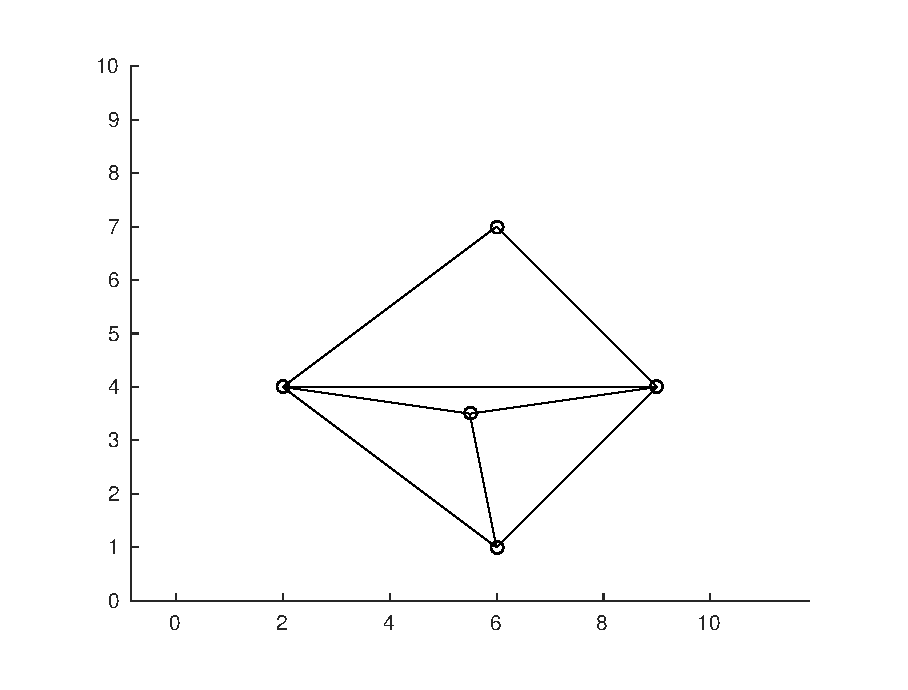
\includegraphics[width=0.4\textwidth]{triangleplane.eps}
\hskip 4pt{\color{Red} \xmark}
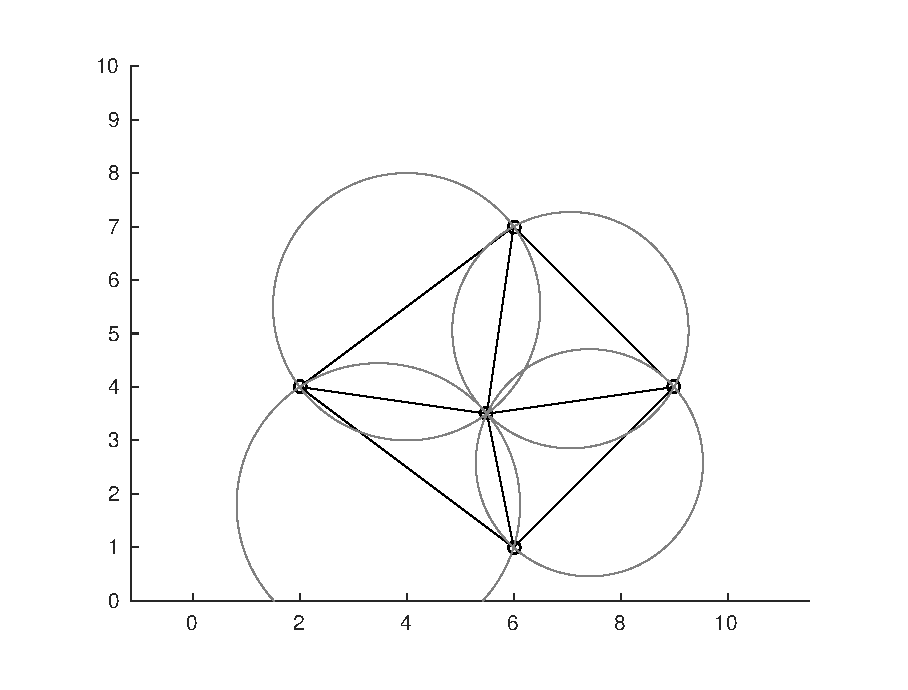
\includegraphics[width=0.4\textwidth]{delaunayplane.eps}
\hskip 4pt{\color{Green} \cmark}
\end{center}
\end{frame}
% Brief applications of Delaunay
\begin{frame}{Delaunay Interpolation}
\textbf{Piecewise linear interpolant:}\\
Let $y \in {\cal S} \in DT({\cal D})$.
${\cal S}$ has vertex set $\{s^{(1)}, \ldots, s^{(d+1)}\}$ and there exist
convex weights $\{w_1, \ldots, w_{d+1}\}$ such that
$y = \sum_{i=1}^{d+1} w_i s^{(i)}$.
$$
{\hat F}_{DT}(y) = \sum_{i=1}^{d+1} w_i F(s^{(i)}).
$$
\medskip
\begin{columns}
\begin{column}{.48\textwidth}
Common interpolation mesh for
\begin{itemize}
\item Finite element method,
\item data science,
\item GIS, and
\item computer graphics
\end{itemize}
\end{column}
\begin{column}{.48\textwidth}
\hbox{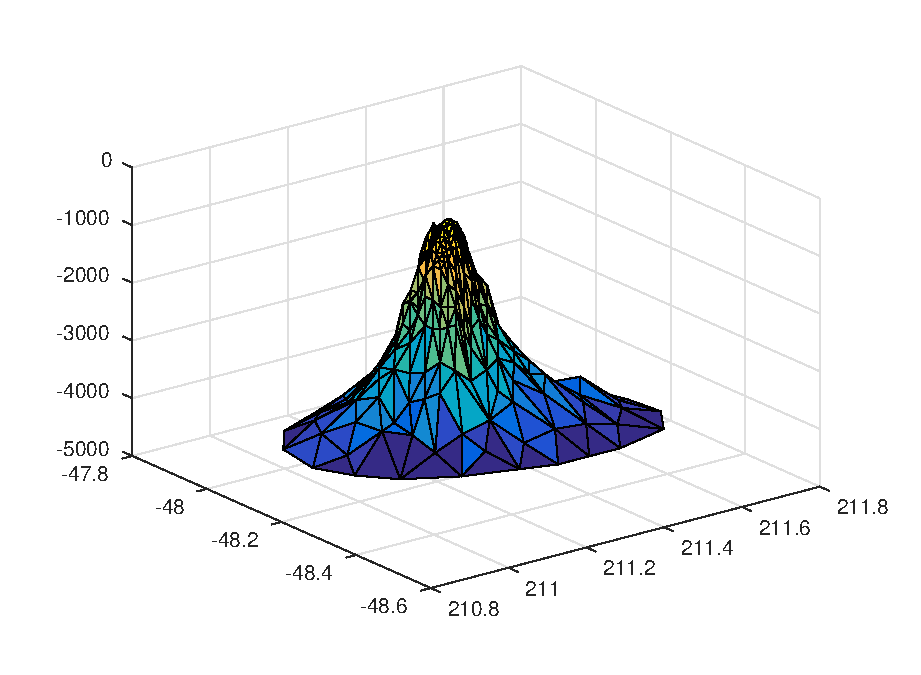
\includegraphics[width=\textwidth]{seamount.eps}}
\end{column}
\end{columns}
\end{frame}
% Some properties of Delaunay that we will need
\begin{frame}{Properties of Delaunay Triangulations}
\begin{itemize}
\item ${\cal D}$ is in {\it general position} when $DT({\cal D})$ exists and
is unique
\begin{itemize}
\item If ${\cal D}$ does not lie in a $(d-1)$-dimensional affine
subspace of $\mathbb{R}^d$, then $DT({\cal D})$ exists
\item If at most $d+1$ points are cospherical, then $DT({\cal D})$ is unique
\end{itemize}
\item Globally Delaunay $\iff$ Locally Delaunay
\item Oweing to Klee, the size of the Delaunay triangulation is
$$
\mathcal{O}\left(n^{\lceil d/2 \rceil}\right)
$$
\pause
\begin{itemize}
\item For $d > 4$, this is expensive!
\item For $d > 8$, this is not scalable!
\end{itemize}
\end{itemize}
\end{frame}
% Interpolation problem
\begin{frame}{Delaunay interpolation}
\textbf{Observation:}
For interpolation at a single point $y$, we only need the
vertices ($\{s^{(1)}, \ldots, s^{(d+1)}\}$) of ${\cal S} \in DT({\cal D})$
such that $y\in {\cal S}$
$$
{\hat F}_{DT}(y) = \sum_{i=1}^{d+1} w_i\text{~}F(s^{(i)}).
$$
\medskip
\textbf{Question:}
Can we find ${\cal S}$ containing $y$ in polynomial time (without computing
the whole Delaunay mesh)?
\end{frame}
% Algorithm description
\subsection{Algorithm for Delaunay interpolation}
% Algorithm for computing the Delaunay interpolant
\begin{frame}{Algorithm outline}
Algorithm to locate Delaunay simplex containing $y$:
\begin{itemize}
\item Grow an initial Delaunay simplex (greedy algorithm) that is
``nearby'' to $y$
\item ``Flip'' accross facets from which $y$ is visible to a new Delaunay
simplex (closer to $y$)
\item This ``visibility walk'' converges to $y$ in finite steps
(Edelsbrunner's acyclicity theorem)
\end{itemize}
\vfill
{\small \it Chang, Watson, Lux, Li, Xu, Butt, Cameron, and Hong.
``A polynomial time algorithm for multivariate interpolation in arbitrary
dimension via the Delaunay triangulation.''
In Proc. 2018 ACMSE Conf.}
\end{frame}
\begin{frame}{Growing the First Simplex}
$\phi$ is the vertex set for the initial Delaunay simplex:
\begin{itemize}
\item Start with $\phi$ containing just the nearest neighbor to $y$ in
${\cal D}$;
\item For all $x \in {\cal D} \setminus \phi$, compute the radius $r_{min}$ of
the smallest circumball about $\{x\} \cup \phi$ and select the $x^*$
that minimizes $r_{min}$;
\item $\phi \leftarrow \phi \cup \{x^*\}$;
\item Repeat until $|\phi| = d+1$;
\end{itemize}
\begin{lemma}
Let ${\cal D}$ be in general position, and
let $\Gamma$ be a Delaunay $j$-face with vertices $\phi \subset {\cal D}$
where $j<d$.
Let $x^* \in {\cal D} \setminus \phi$
minimize the radius of the smallest $(d-1)$-sphere through the points in
$\phi \cup \{x\}$, over all $x \in {\cal D} \setminus \phi$.
Then $\Gamma^* = \text{ConvexHull}(\phi \cup \{x^*\})$ is a Delaunay
$(j+1)$-face.
{\bf Proof in Thesis.}
\end{lemma}
\end{frame}
% How to flip across an open facet
\begin{frame}{Flipping}
\begin{columns}
\begin{column}{.58\textwidth}
\begin{itemize}
\item Let $\phi$ be the vertices for a facet of a Delaunay simplex;
\item Let $\Gamma$ be the facet with vertices in $\phi$;
\item Let ${\cal H}$ be the halfspace containing $y$,
w.r.t. the hyperplane containing $\Gamma$
\item Unless $\Gamma$ is a facet of the convex hull, there exists
$x^* \in {\cal D} \setminus \phi$ such that $\phi \cup \{x^*\}$
is the vertex set for a Delaunay simplex;
\end{itemize}
\end{column}
\begin{column}{.4\textwidth}
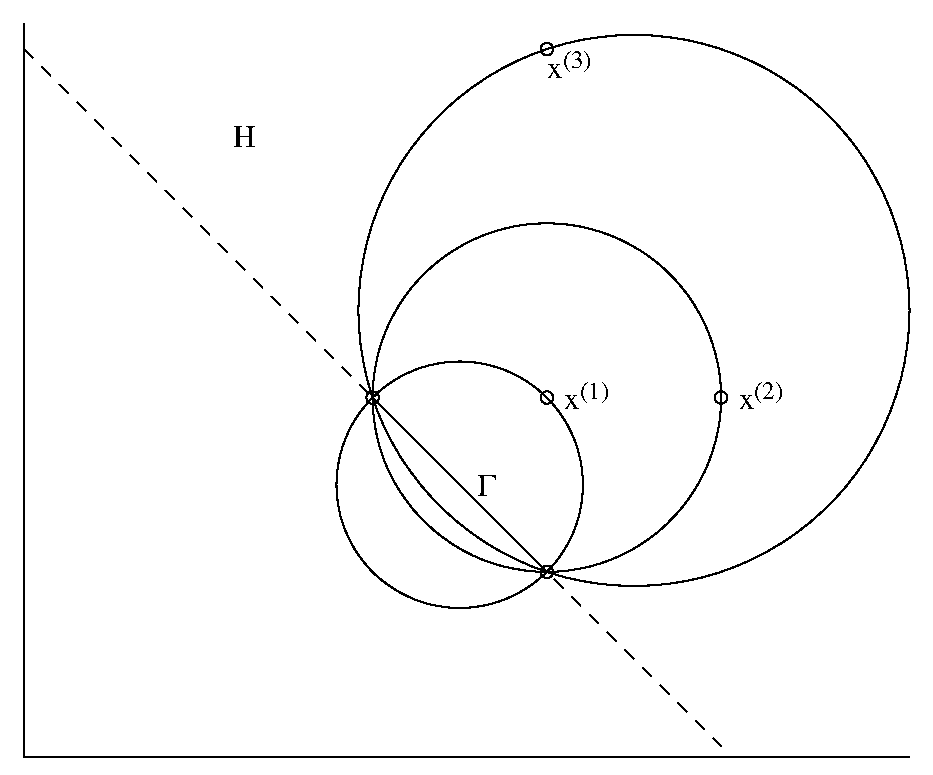
\includegraphics[width=\textwidth]{circles.eps}
\end{column}
\end{columns}
\medskip
\centerline{\bf Proof in Thesis.}
\end{frame}
% The visibility walk
\begin{frame}{Visibility walk}
\begin{columns}
\begin{column}{.48\textwidth}
\begin{itemize}
\item Grow an initial simplex ${\cal S}^{(0)}$;
\item While $y \not\in {\cal S}^{(k)}$, generate $S^{(k+1)}$ by flipping
across a facet of $S^{(k)}$ from which $y$ is ``visible'';
\item Terminate when $y\in {\cal S}^{(k)}$, otherwise, $k \leftarrow k+1$;
\end{itemize}
\end{column}
\begin{column}{.48\textwidth}
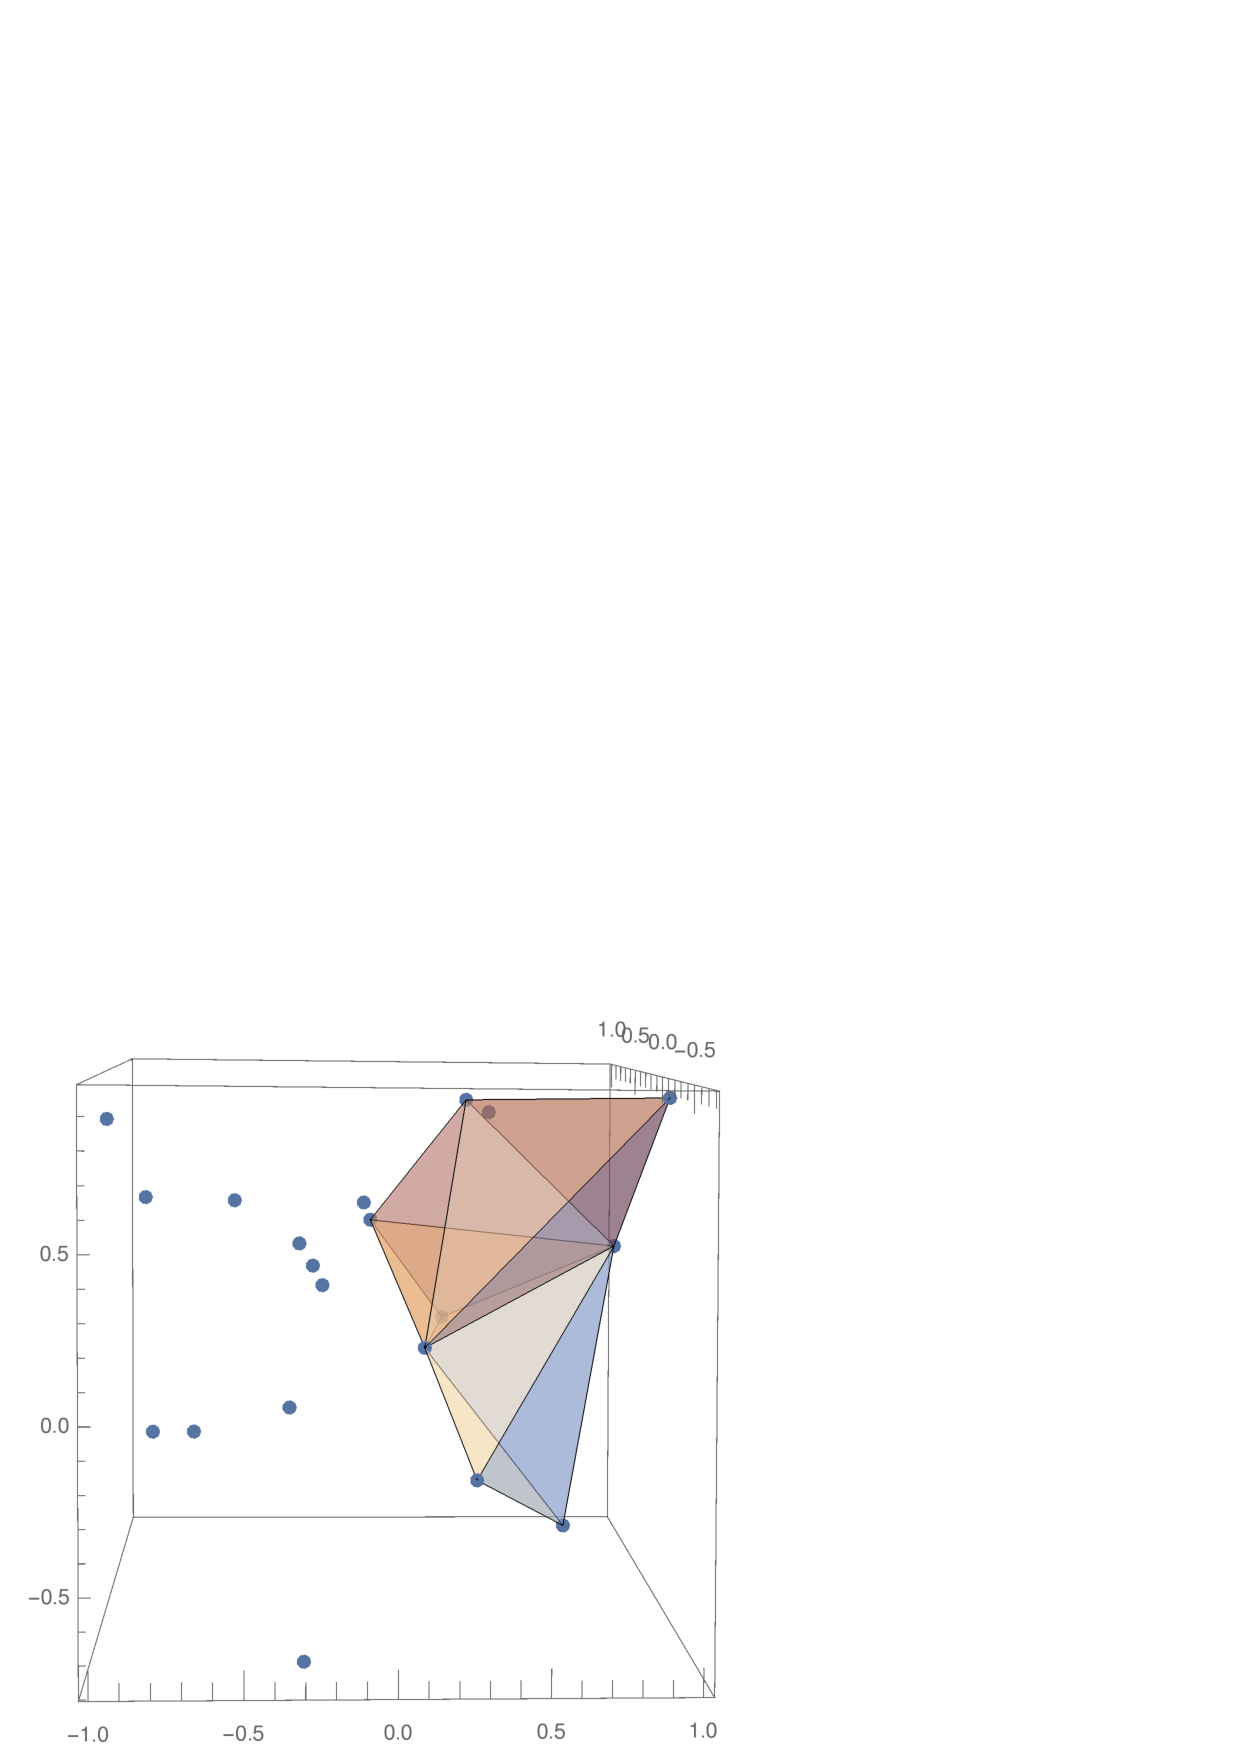
\includegraphics[width=\textwidth]{DelaunayWalk.pdf}
\end{column}
\end{columns}
\medskip
Converges in finite flips by {\it Edelsbrunner's Acyclicity Theorem}.
\end{frame}
% Complexity
\begin{frame}{Algorithm Complexity}
\begin{itemize}
\item To grow the first simplex:
$\mathcal{O}(n d^3)$ to apply $n$ rank-1 updates to the QR factorization of
$d \times j$ matrix for $j=1,\ldots,d$
\item To compute a flip:
$\mathcal{O}(n d^2)$ to apply $n$ rank-1 updates to the QR factorization of
a $d \times d$ matrix
\item $\ell$ total flips\\
\centerline{\small
\begin{tabular}{l|cccc}
  & $n=2K$ & $n=8K$ & $n=16K$ & $n=32K$\\
\hline
$d=2$  & 3.05 & 2.90 & 3.25 & 3.10\\
$d=8$  & 23.75 & 24.75 & 24.30 & 23.10\\
$d=32$ & 95.25 & 125.60 & 131.85 & 150.10\\
$d=64$ & 171.95 & 221.85 & 248.35 & 280.60\\
\end{tabular}}
\end{itemize}
\medskip
\pause
{\bf Overall complexity:} $\mathcal{O}(nd^2 \ell)$\\
\medskip
\pause
{\bf Unresolved question:} $\ell \approx d$? $\ell$ independent of $n$?
\end{frame}
% Linear programming
\begin{frame}{Linear programming interpretation}
$$
{\tilde A} = \left[ \begin{matrix}
(-x^{(1)})^T & 1 \cr
(-x^{(2)})^T & 1 \cr
\vdots & \vdots \cr
(-x^{(n)})^T & 1 \cr
\end{matrix}\right]\text{, }
{\tilde b} = \left[ \begin{matrix}
\| x^{(1)} \|_2^2 \cr
\| x^{(2)} \|_2^2 \cr
\vdots \cr
\| x^{(n)} \|_2^2 \cr
\end{matrix}\right]\text{, and }
{\tilde c} = \left[ \begin{matrix}
-y \cr
1 \cr
\end{matrix}\right].
$$
\pause
$\displaystyle \hbox{\bf Primal prob: }
\max_{\tilde u} {\tilde c}^T {\tilde u}
\hbox{ such that }
{\tilde A}{\tilde u} \lee {\tilde b}, {\tilde u}\hbox{ free}.$\\
{\bf Ext pts:}
${\tilde u} = (-2\hbox{circumcenter}, \hbox{circumradius}^2 - \|\hbox{circumcenter}\|_2^2)$\\
\medskip
\pause
$\displaystyle \hbox{\bf Dual prob: }
\min_{\tilde v} {\tilde b}^T {\tilde v}
\hbox{ such that }
{\tilde A}^T{\tilde v} = {\tilde c}, {\tilde v}\gee 0.$\\
{\bf Ext pts:}
$\Rightarrow$ ${\tilde v}$ are convex weights for $y$\\
\medskip
\pause
Primal + dual feasible $\Rightarrow$ Delaunay simplex containing $y$\\
\medskip
\pause
{\bf LP basic solution in polynomial time is an open problem!}
\end{frame}
% Extrapolation
\begin{frame}{Extrapolation}
What about extrapolation?
\begin{itemize}
\item Project $y$ on to the convex hull of ${\cal D}$
\item Interpolate the projection (if the residual is small)
\item Note: projection is a quadratic program (more expensive than an LP)
\end{itemize}
Let $E$ be a $d\times n$ matrix whose columns are points in ${\cal D}$, and let
$z$ be an extrapolation point (outside convex hull of $P$).
$$
\xi^* = \arg\min_{\xi\in\mathbb{R}^n} \|E\xi - z\| \quad\hbox{subject to}\quad
\xi \ge 0 \quad\hbox{and}\quad \sum_{i=1}^n \xi_i = 1.
$$
Projection: ${\hat z} = E\xi^*$
\end{frame}
% Implementation description
\subsection{Serial implementation}
% DELAUNAYSPARSE
\begin{frame}{DELAUNAYSPARSE Package}
Standalone software package {\tt DELAUNAYSPARSE}:
\begin{itemize}
\item Robust against degeneracy
\item Runs in $\mathcal{O}(m n d^2 \ell)$ time, where $\ell$ is the
number of ``flips'', $n$ is the numer of data points, $d$ is the dimension,
and $m$ is the number of interpolation points
\item Typically, $\ell \approx \mathcal{O}(d)$ or $\mathcal{O}(d\log d)$
(linear in $n$)
\item Parallel and serial implementations
\end{itemize}
\vfill
{\small \it Chang, Watson, Lux, Butt, Cameron, and Hong.
``Algorithm XXX: DELAUNAYSPARSE: Interpolation via a sparse subset of the
Delaunay triangulation in medium to high dimensions.''
Submitted to ACM Transactions on Mathematical Software (2019)}. 
\end{frame}
% Serial performance
\begin{frame}{Serial performance}
Runtime in seconds for interpolating a single point ($m=1$) with $n$ points
in $d$ dimensions\\
\bigskip
\medskip
\begin{tabular}{c|ccccc}
& & & $d$ & & \\
$n$ & 2 & 8 & 32 & 64 & 128 \\
\hline
250    & 0.005  & 0.013   & 0.150   & 3.404    & 27.078   \\
500    & 0.021  & 0.042   & 0.325   & 6.479    & 59.511   \\
1000   & 0.083  & 0.152   & 0.791   & 14.020   & 124.320  \\
2000   & 0.344  & 0.583   & 2.230   & 28.984   & 242.066  \\
4000   & 1.314  & 2.284   & 7.165   & 62.494   & 502.620  \\
8000   & 5.580  & 9.027   & 26.210  & 151.177  & 905.711  \\
16,000 & 22.086 & 35.725  & 109.448 & 386.596  & 2190.362 \\
32,000 & 82.915 & 145.115 & 421.934 & 1097.060 & 5024.675 \\
\end{tabular}
\end{frame}
% Parallel implementation
\subsection{Parallel implementation}
\begin{frame}{Parallel implementation}
\textbf{Distributed memory:} Trivial, for $m > 1$, just run
the serial algorithm with multiple batches of interpolation points
${\cal Q} = {\cal Q}^{(1)} \cup {\cal Q}^{(2)} \cup \ldots$\\
\medskip
{\bf Shared memory:} Multiple levels
\begin{itemize}
\item Level 1: shared memory loop over multiple interpolation points (just
like the distributed case)
-- Add a few locks in order to ``check ahead'' if the current simplex
contains future interpolation points
\item Level 2: loop(s) over data points -- results in additional work to
reduce multiple solutions; preferrable only when $m$ is small and $n$ is large
\end{itemize}
\end{frame}
% Parallel performance
\begin{frame}{Parallel performance}
\begin{center}
\includegraphics[width=0.7\textwidth]{parallelBigD.eps}\\
$d=50\text{, }n=500\text{, }m=64$
\includegraphics[width=0.7\textwidth]{parallelBigM.eps}\\
$d=10\text{, }n=1000\text{, }m=1024$
\end{center}
\end{frame}

% Pause/reset
\begin{frame}{Transition to VTMOP}
\tableofcontents
\end{frame}

% VTMOP section
\section{VTMOP package}
% Symbols/terminology
\begin{frame}{Review of Nomenclature}
\begin{itemize}
\item Predict/optimize the function $F : \mathbb{R}^d\rightarrow\mathbb{R}^p$
\item $x,y,z$ will denote arbitrary points in $\mathbb{R}^d$;
\item For real $n$-tuples $u,v$:
\begin{itemize}
\item $u < v$ if $u$ is componentwise strictly less than $v$;
\item $u \lee v$ if $u$ is componentwise less than or equal to $v$;
\item $u \leq v$ if $u \lee v$ with strict inequality in at least one component;
\end{itemize}
\item $i,j$ are indices;
\begin{itemize}
\item $u^{(i)}_j$ is the $j$th component of the $i$th vector in some list;
\end{itemize}
\pause
\item $X,Y,Z$ will denote arbitrary points in $\mathbb{R}^p$;
\item $F = (f_1, \ldots, f_p)$, where $f_i(x) : \mathbb{R}^d \rightarrow \mathbb{R}$
\item $\mathbb{R}^d$ is the {\it design space} and $\mathbb{R}^p$ is the {\it objective space};
\item $\mathcal{X} = [L,U]$ is the feasible design space;
\item $\mathcal{Y} = F(\mathcal{X})$ is the feasible objective space;
\end{itemize}
\end{frame}

\subsection{Blackbox MOPs}
% Formal definitions
\begin{frame}{Formal MOP Definition}
\begin{itemize}
\item The MOP attempts to balance the tradeoff between multiple conflicting
objectives;
\item The solution to a MOP is a set of {\it nondominated} or
{\it Pareto optimal} solutions;
\item $x^*$ is Pareto optimal if for all $x\in\mathcal{X}$, $F(x) \not\leq F(x^*)$;
\begin{center}
\includegraphics[width=0.45\textwidth]{feasible_design.eps}
\includegraphics[width=0.45\textwidth]{convex_pareto.eps}
\end{center}
\end{itemize}
\end{frame}

% Pareto/efficient defn
\begin{frame}{Goals:}
\begin{center}
\begin{tabular}{|ccc|}
\hline
&&\\
&{\large Find a discrete set of approximately}&\\
&{\large nondominated objective points that}&\\
&{\large describes the Pareto front, and the}&\\
&{\large corresponding efficient designs}&\\
&&\\
\hline
\end{tabular}
\end{center}
\end{frame}
% Blackbox problems
\begin{frame}{Expensive Blackbox MOPs}
\begin{center}
{\bf Types of MOPs}\\
\smallskip
{\footnotesize
\begin{tabular}{|c|c|}
\hline
\begin{tabular}{c}
 \\
functions are ``cheap'' to evaluate\\
derivative info is available\\
\\
\end{tabular}
& 
\begin{tabular}{c}
 \\
functions are ``cheap'' to evaluate\\
no derivative info is available\\
\\
\end{tabular}\\
\hline
\begin{tabular}{c}
\\
functions are costly to evaluate\\
derivative info is available\\
\\
\end{tabular}
&
\begin{tabular}{c}
\\
functions are costly to evaluate\\
no derivative info is available\\
\\
\end{tabular}\\
\hline
\end{tabular}
}
\end{center}
\medskip
Focus on bottom right: {\bf expensive blackbox MOPs}!
\end{frame}
% Problem difficulties
\begin{frame}{Spectrum of blackbox problems}
Computationally cheap $\xrightarrow{\hspace*{4cm}}$ expensive
\bigskip
\begin{columns}
\begin{column}{.33\textwidth}
\begin{itemize}
\item Eval: $\approx$ secs
\item Budget: $\approx 10,000$s
\item Software: {\tt NSGA-II}
\end{itemize}
\end{column}
\begin{column}{.33\textwidth}
\begin{itemize}
\item Eval: $\approx$ mins
\item Budget: $\approx 1000$s
\item Software: {\tt VTMOP}
\end{itemize}
\end{column}
\begin{column}{.33\textwidth}
\begin{itemize}
\item Eval: $\approx$ hrs
\item Budget $\approx 100$ (at most)
\item Software: {\tt FUN3D}? {\tt NASTRAN}?
\end{itemize}
\end{column}
\end{columns}
\end{frame}
%% Common techniques
%\begin{frame}{Common techniques}
%\begin{itemize}
%\item Multiobjective Evolutionary Algorithms
%\begin{itemize}
%\item Requires many function evaluations
%\item Random by nature
%\end{itemize}
%\item Multiobjective Direct Search
%\begin{itemize}
%\item Mainly for biobjective case
%\end{itemize}
%\item Scalarization
%\begin{itemize}
%\item Reduce MOP to SOP using scalarization function
%\item Solve many scalarized subproblems
%\end{itemize}
%\end{itemize}
%\end{frame}
%% Weighted sum
%\begin{frame}{Weighted Sum Method}
%$$
%\min_{x\in\mathcal{X}}\text{ } w^T F(x) \text{, for } w \succeq \Vec{0}
%$$
%\begin{itemize}
%\item For $w > \Vec{0}$, the solution is Pareto optimal
%\item An {\it adaptive weighting scheme} is required
%\item Cannot produce solutions in nonconvex regions of Pareto front\\
%$\qquad\qquad$
%\includegraphics[width=0.5\textwidth]{nonconvex_pareto.eps}
%\end{itemize}
%\end{frame}
%% RSM
%\begin{frame}{The Response Surface Methodology}
%\begin{itemize}
%\item Do an experimental design, use design to fit ``cheap'' surrogate models,
%use surrogates to predict optimal designs
%\item Very economic for blackbox problems
%\item Useful for MOP since the models can be reused for multiple
%scalarizations
%\end{itemize}
%\end{frame}

% Main proposal section
\subsection{A Multiobjective Optimization Algorithm}
% Introducing VTMOP solver...
\begin{frame}{VTMOP}
\texttt{VTMOP} is a Fortran 2008 blackbox MOP solver and framework,
based on an algorithm by\\
\medskip
{ \small \it Deshpande, Watson, and Canfield.
``Multiobjective optimization using an adaptive weighting scheme.''
Optimization Methods and Software (2016).}\\
\medskip
Combines adaptive weighting scheme, response surface modeling, and trust
region methods
\end{frame}
% Describing Shubhangi's algorithm
\begin{frame}{The Algorithm Outline}
\begin{center}
\includegraphics[width=0.95\textwidth]{algorithm-chart.pdf}
\end{center}
\end{frame}
% Describing Shubhangi's algorithm
\begin{frame}{RSM phases}
\begin{center}
\includegraphics[width=0.95\textwidth]{rsm-chart.png}
\end{center}
\end{frame}
% Describing Shubhangi's algorithm
\begin{frame}{0th iteration}
\begin{center}
\includegraphics[width=0.95\textwidth]{0thit-chart.png}
\end{center}
\end{frame}
% Describing Shubhangi's algorithm
\begin{frame}{Key component}
\begin{center}
\includegraphics[width=0.95\textwidth]{isolated-chart.png}
\end{center}
\end{frame}
% Identifying an isolated point
\begin{frame}{Identifying an Isolated Point}
Let $P^{(k)}$ be the $k$th set of nondominated objective points
$P^{(k)} = \{X^{(1,k)}, \ldots, X^{(M^{(k)},k)}\} $.
\medskip
Define the projected set 
$$
\Pi^{(k)} = \left\{ \left(\frac{X^{(i,k)}_1}{X^{(i,k)}_p}, \ldots,
\frac{X^{(i,k)}_{p-1}}{X^{(i,k)}_p}\right) \quad\bigg|\quad
i = 1, \ldots, M^{(k)}\right\}
$$
The most isolated point is identified by considering the average
Euclidean distance to all neighbors in the Delaunay graph of $\Pi^{(k)}$\\
\begin{center}
\includegraphics[width=.5\textwidth]{del-nbhd.png}\\
{\it Image from Wikipedia}
\end{center}
\end{frame}
% Getting the Delaunay graph
\begin{frame}{Getting the Delaunay Graph}
\textbf{Compute the Delaunay neighborhood} of $X^{(1,k)}$, $\ldots$,
$X^{(M^{(k)},k)}$ with respect to the projected set $\Pi^{(k)}$.\\
\medskip
\begin{itemize}
\item Using current state-of-the-art Delaunay graph algorithm in CGAL,
requires exponential time to compute
\item But, we only need the Delaunay graph $DG(\Pi^{(k)})$
\item The number of connections in $DG(\Pi^{(k)})$ is upper bounded by
$M^{(k)}(M^{(k)}-1)/2$
\item Can recover $DG(\Pi^{(k)})$ by interpolating the midpoint between each
pair of points in $\Pi^{(k)}$
\item Using {\tt DELAUNAYSPARSE}, requires
$\mathcal{O}((M^{(k)})^3 p^2 \ell)$ time
\end{itemize}
\smallskip
\centerline{\bf Proof in Thesis}
\end{frame}

\subsection{VTMOP as a General Framework}
\begin{frame}{A Framework for Multiobjective Optimization}
\begin{enumerate}
\item
If $k>0$, identify an
isolated point $F({\tilde x}^{(k)})$ in the
current nondominated set; center the $k$th LTR $\Delta^{(k)}$ about
${\tilde x}^{(k)}$; and assign the $k$th set ${\cal W}^{(k)}$ of
adaptive weights.
If $k=0$, then 
$\Delta^{(0)} = [L,U]$ and ${\cal W}^{(0)}$ is assigned predetermined values
\item
Perform the $k$th exploration by sampling $F$ within $\Delta^{(k)}$
\item
Fit $p$ surrogates, ${\hat f}^{(k)}_i \approx f_i$ for
$i=1$, $\ldots$, $p$,
using the data gathered from Step 2 (plus any data available from previous
iterations).
Apply each weight vector in ${\cal W}^{(k)}$ to ${\hat f}^{(k)}_1$, $\ldots$,
${\hat f}^{(k)}_p$,
and minimize the resulting surrogates using a local optimizer to get
the $k$th batch ${\cal C}^{(k)}$ of candidate designs
\item
Evaluate $F(z)$ for all $z \in {\cal C}^{(k)}$.
Increment $k$.
Update the current database of function values, check for termination
conditions, and proceed
to the next iteration
\end{enumerate}
\end{frame}
% Section on Parallel versions
\subsection{Parallel implementation}
% Source of parallelism
\begin{frame}{Sources of Parallelism}
\begin{enumerate}
\item The function $F$ (left to the user)
\item Iteration complexity (assumed to not offer much improvement)
\item Function evaluations $\leftarrow$ {\bf most important}
\end{enumerate}
\end{frame}
% Describing Shubhangi's algorithm
\begin{frame}{Function evaluations}
\begin{center}
\includegraphics[width=0.95\textwidth]{eval-chart.png}
\end{center}
\end{frame}
% How to use parallelism
\begin{frame}{Parallelizing the original algorithm}
\begin{itemize}
\item Recall that $F$ is being distributed by user
\item Use OpenMP {\it shared memory parallelism}, essentially for achieving
asynchronous behavior
\item Puts burden of distribution on user
\item Better flexibility for real-world HPC systems
\end{itemize}
\medskip\pause
To parallelize function evaluations:
\begin{itemize}
\item Batch of candidates can be trivially evaluated in parallel
\item Instead of using {\tt pVTdirect} from VTDIRECT95 (which uses MPI)
made a modification to the serial code called {\tt bVTdirect} that evaluates
batches of points in parallel using OpenMP
\item For maximal parallelism, replace {\tt bVTdirect} with a Latin hypercube
design, which can be evaluated in parallel
\end{itemize}
\end{frame}
% LibEnsemble
\begin{frame}{libEnsemble}
The {\tt libEnsemble} library is part of the Exascale Computing
Project at Argonne to harness increased levels of concurrency
when distributing large simulations over extreme scale resources
\begin{itemize}
\item Generator function (generates simulations to run)
\item Simulator function (runs simulations, possibly in parallel)
\item Allocator function (decides whether to generate or simulate)
\end{itemize}
\bigskip
\pause
\texttt{VTMOP} is the {\it generator} for {\tt libEnsemble}
\begin{itemize}
\item Each call to the {\it generator} runs a half-iteration and requests
a design exploration (using Latin hypercube) or a batch of candidate evaluations
\item The {\it simulator} evaluates all the requested designs
\item The {\it allocator} waits until all designs are evaluated and then
swithes back to the {\it generator}
\end{itemize}
\end{frame}
% LibEnsemble
\begin{frame}{Integrating with libEnsemble}
\begin{itemize}
\item Want nice big batches that match available resources
\item Use a Latin hypercube search during the search phase
\item Pad out batches of candidates using additional weights
\end{itemize}
\begin{center}
\includegraphics[width=0.7\textwidth]{eval-chart.png}
\end{center}
\end{frame}
% Test functions
\begin{frame}{Test functions}
\begin{columns}
\begin{column}{.58\textwidth}
\begin{itemize}
\item $F^{(c)}(x) = (\|x - 0.5e^{(1)}\|_2^2, \ldots, \|x - 0.5e^{(p)}\|_2^2)$
\item Convex Pareto front $\Rightarrow$ ``easier'' problem
\end{itemize}
\bigskip\bigskip
\begin{itemize}
\item {\tt DTLZ2} from Deb et al.
\item Concave Pareto front $\Rightarrow$ ``harder'' problem
\end{itemize}
\end{column}
\begin{column}{.4\textwidth}
\bigskip
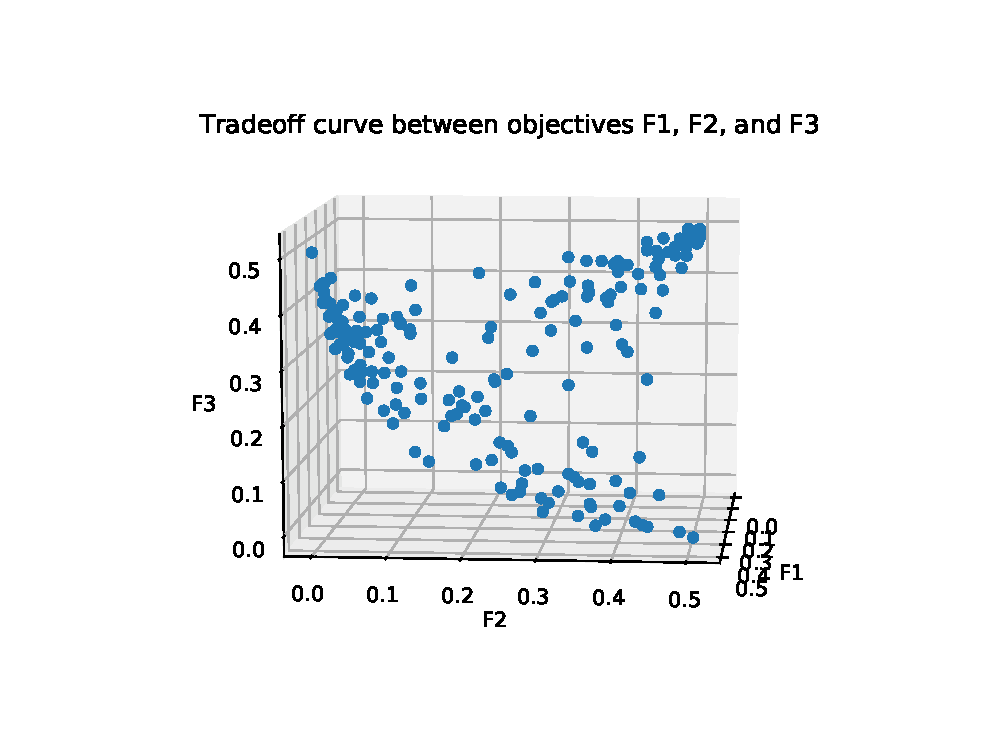
\includegraphics[width=\textwidth]{f_conv_2.eps}\\
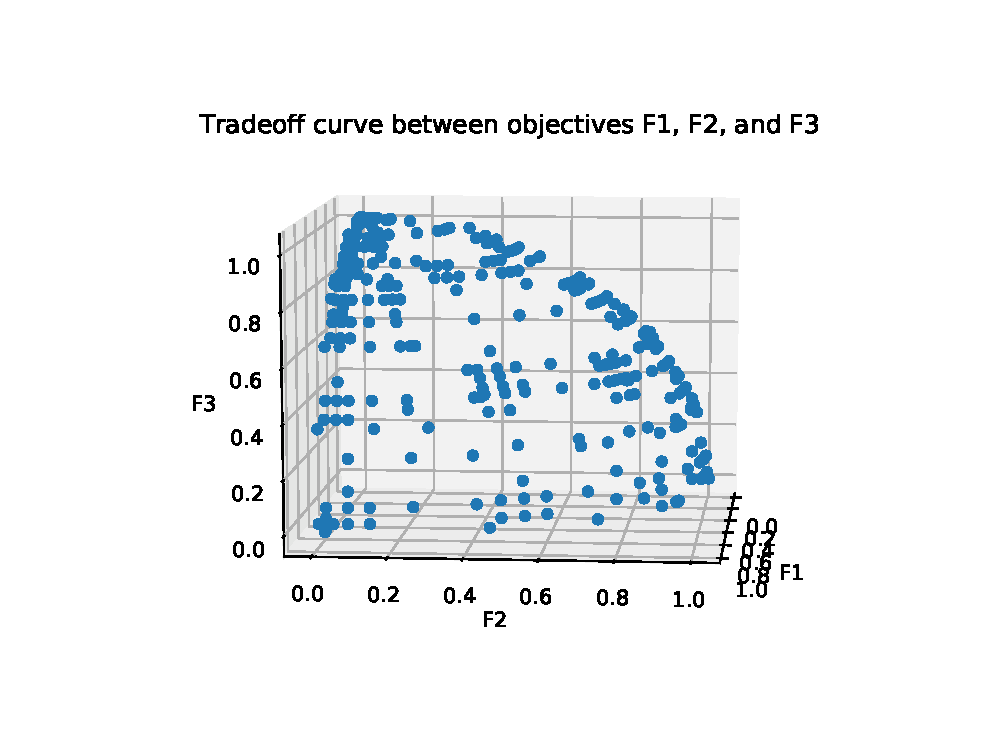
\includegraphics[width=\textwidth]{dtlz2_2.eps}
\end{column}
\end{columns}
\end{frame}
\begin{frame}{Performance metrics}
Evaluating a multiobjective optimization solution is a multiobjective
problem...\\
\medskip
We want:
\begin{enumerate}
\item Many points on the Pareto front (measured by {\it cardinality} of the
solution set)
\item Good convergence of the solution points to the true Pareto front
(measured by RMSE)
\item Even  spacing/good coverage of the solution set
(measured by Delaunay discrepancy, computed with {\tt ScipPy})
\end{enumerate}
\end{frame}
% Performance results
\begin{frame}{Approximation results (2000 evaluations)}
Average (5 runs) number of solutions, RMSE, and Delaunay discrepancy
for $F^{(c)}$ and {\tt DTLZ2} with $d=5$ for VTMOP using {\tt bVTdirect} (DIR),
Latin hypercube search (LH),
and {\tt libEnsemble} (LIBE)\\
\begin{center}
{\small
\begin{tabular}{c|ccc}
Prob/Meth&$p=2$&$p=3$&$p=4$\\
\hline
{$F^c$ / DIR\hskip 4pt} & 73, .00100, .207 & 173, .0505, .579 & 288, .101, NA\\
{$F^c$ / LH\hskip 8pt} & 38, .0115, .180 & 93, .0665, .512 & 171, .117, .689\\
{$F^c$ / LIBE } & 78, .0127, .158 & 189, .0560, .429 & 283, .104, .551\\
\hline
{{\tt DTLZ2} / DIR\hskip 4pt} & 139, .00713, .109 & 354, .0401, .230 & 658, .0443, NA\\
{{\tt DTLZ2} / LH\hskip 8pt} & 80, .0993, .139 & 264, .167, .458 & 510, .210, .757\\
{{\tt DTLZ2} / LIBE } & 66, .103, .201 & 258, .175, .691 & 548, .201, .793\\
\end{tabular}
}
\end{center}
NA = Missing values due to {\tt SciPy}'s Delaunay triangulation tool
\end{frame}
% Runtimes
\begin{frame}{Runtime performance (2000 evaluations)}
CPU time / wall time in seconds for DIR, LH, and LIBE versions
with 36 cores \& 1 sec (+ var)/1 core per eval\\
\medskip
\centerline{\small
\begin{tabular}{cc|cccc}
$p$ & Meth & $F^{(c)}$ no var & $F^{(c)}$ + var & {\tt DTLZ2} no var
& {\tt DTLZ2} + var\\
\hline
& DIR & 2008 / 1037 & 2007 / 1039 & 2007 / 1093 & 2004 / 1082\\
$2$ & LH & 2015 / 89 & 2017 / 107 & 2028 / 89 & 2011 / 109\\
%& {\tt bVTdir2} & NA / 170 & NA / 239 & NA / 175 & NA / 240\\
& LIBE & 2051 / 112 & 2070 / 142 & 2060 / 111 & 2064 / 143\\
\hline
& DIR & 2012 / 717 & 2012 / 719 & 2021 / 797 & 2018 / 797\\
 $3$ & LH & 2023 / 94 & 2034 / 116 & 2040 / 95 & 2023 / 117\\
%& {\tt bVTdir2} & NA / 137 & NA / 207 & NA / 165 & NA / 237\\
& LIBE & 2077 / 133 & 2066 / 144 & 2054 / 99 & 2057 / 126\\
\hline
& DIR & 2026 / 582 & 2029 / 586 & 2177 / 807 & 2149 / 782\\
$4$ & LH & 2042 / 108 & 2045 / 127 & 2176 / 200 & 2201 / 280\\
%$4$ & {\tt bVTdir2} & NA / 134 & NA / 208 & NA / 280 & NA / 348\\
& LIBE & 2134 / 190 & 2124 / 186 & 2182 / 227 & 2185 / 257\\
\end{tabular}}
\medskip

{\it \small Chang, Larson, Watson, and Lux.
``Managing computationally expensive blackbox multiobjective optimization
problems with libEnsemble.''
To appear in SpringSim 2020, 28th HPC Symposium.}
\end{frame}
% show CPU usage plots
\begin{frame}{CPU Usage (36 cores)}
\begin{center}
\includegraphics[width=.4\textwidth]{vtdir_cpu_plt.eps}\\
{\small DIR (not suitable for $36$ cores)}\\
\includegraphics[width=.4\textwidth]{libe1_cpu_plt.eps}\hskip 20pt
\includegraphics[width=.4\textwidth]{libe2_cpu_plt.eps}\\
{\small\hskip 10pt LH \hskip 130pt LIBE}
\end{center}
\end{frame}

% Pause/reset
\begin{frame}{Applications}
\tableofcontents
\end{frame}

% Applications and future work
\section{Applications and future work}
% VarSys problem
\begin{frame}{The VarSys Problem}
\textbf{VarSys:} Managing performance variance
\begin{itemize}
\item For multiple runs of the same task on the same HPC system,
we get varying performance (i.e., throughputs)
\item This presents issues for load balancing and performance guarantees
\item Needs to be balanced against other concerns such as energy consumption
and mean throughput
\item Evaluation expense: 1+ minutes to build approximations to throughput
distribution
\end{itemize}
\end{frame}

\subsection{Predicting Performance Variability with DELAUNAYSPARSE}
% Summary of variability map prediction
\begin{frame}{Step 1: Predicting with DELAUNAYSPARSE}
\begin{itemize}
\item First goal is to construct a {\it variability map} for predicting
I/O throughput variablity
\item Model I/O variability as a function of number of threads, CPU freq,
file size of I/O operation, and record size of file system (4 variables total)
\item Perform 40 runs of {\tt IOzone} benchmark at each configuration in an
experimental design
\item Compute variability at each design based on 40 runs of {\tt IOzone}
\item Fit a Delaunay model to predict variability for new system
configurations
\end{itemize}
\end{frame}
% Summary of collaborators' work
\begin{frame}{Why Delaunay?}
Collaborators' works show that Delaunay interpolation outperforms
other techniques (e.g., neural network, support vector regressor,
{\tt LSHEP}, and multivariate splines) for constructing variability map
\begin{itemize}
\item
{\it \small Cameron et al. ``MOANA: Modeling and analyzing I/O variability in
parallel system experimental design.'' IEEE Trans. Parallel and Distrib. Systems
(2019)}
\item
{\it \small Lux, Watson, Chang, Hong, and Cameron.
``Interpolation of sparse high-dimensional data.''
Submitted to Numerical Algorithms (2019).}
\item
{\it \small Lux et al.
``Predictive modeling of I/O characteristics in high performance
computing systems.''
In Proc. SpringSim 2018, the 26th HPC Symp.}
\item
{\it \small Lux et al.
``Nonparametric distribution models for predicting and managing computational
performance variability.''
In Proc. IEEE SoutheastCon 2018}
\end{itemize}
\end{frame}
% Convergence plot on VarSys problem
\begin{frame}{DELAUNAYSPARSE Convergence on VarSys}
\centerline{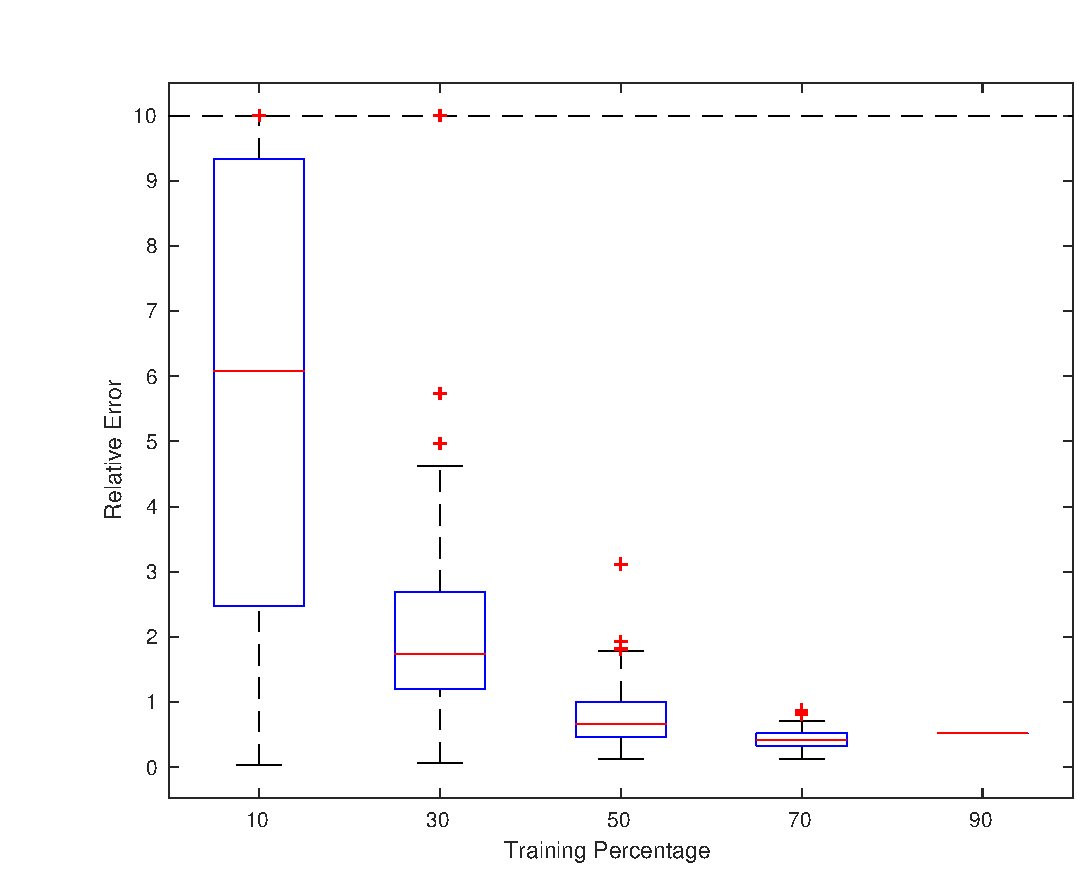
\includegraphics[width=.4\textwidth]{q2.eps}\hskip 20pt
\includegraphics[width=.4\textwidth]{q3.eps}}
\centerline{Convergence with increasing data for 2 points in holdout set}
\medskip
{\it \small Chang, Watson, Lux, Bernard, Li, Xu, Back, Butt, Cameron, and Hong.
``Predicting system performance by interpolation using a high-dimensional
Delaunay triangulation.'' In Proc. SpringSim 2018, the 26th HPC Symp.}
\end{frame}

\subsection{Managing Performance Variability with VTMOP}
% Summary of variability optimization
\begin{frame}{Step 2: Controlling with VTMOP}
\begin{itemize}
\item Now turn to compute bound tasks and use {\tt HPL} benchmark
(used for Top500 list)
\item Want to manage performance variability synergystically with mean
performance
\item Tune 5 parameters for {\tt HPL} on HPC system {\tt Bebop} at Argonne
\item Maximize mean throughput, minimize throughput standard deviation
\item Ran {\tt HPL} 30 times on 4 nodes with 36 cores per node and a problem
size of $20,000$ for each evaluation
\end{itemize}
\end{frame}
% Results of tuning HPL
\begin{frame}{Results of HPL Tuning}
The ``recommended'' setting was not Pareto optimal
\begin{itemize}
\item Came close to fastest times in mean throughput (2.24 Tflops)
\item 4 times higher standard deviation (21.4 Gflops)
\end{itemize}
\centerline{\includegraphics[width=.55\textwidth]{hpl_n20k_pf.eps}}
\medskip
{\it \small Chang, Larson, and Watson.
``Multiobjective optimization of the variability of the high-performance
LINPACK solver.'' Submitted to 2020 Winter Simulation Conf.}
\end{frame}

% Summary of future works
\subsection{Future Work}
\begin{frame}{Summary of Contributions}
\begin{itemize}
\item A novel algorithm for Delaunay interpolation in high dimensions
\item DELAUNAYSPARSE software package implementing this algorithm
\item A novel algorithm for computing the Delaunay graph
\item VTMOP software package and framework for solving MOPs
\item 3 ways to get parallelism with VTMOP
\item Predicting \& managing variability using DELAUNAYSPARSE and VTMOP
\end{itemize}
\end{frame}
% Future work for DELAUNAYSPARSE
\begin{frame}{Future Work for DELAUNAYSPARSE}
\begin{itemize}
\item A neural network that uses ReLU activation with zero training error is
also a piecewise linear interpolant, but in literature, Delaunay interpolant
is often considered to be an ``optimal'' piecewise linear interpolant
\item Delaunay triangulation is defined for an arbitrary metric space.
Can Delaunay interpolation be done in high-dimensional arbitrary metric space?
\item Other subsets of the Delaunay triangulation:\\
{\it \small Chang, et al. 
``Computing the umbrella neighbourhood of a vertex in the Delaunay 
triangulation and a single Voronoi cell in arbitrary dimension.''
In Proc. IEEE SoutheastCon 2018.}
\item Distributed memory version of DELAUNAYSPARSE
\end{itemize}
\end{frame}
% Future work for VTMOP
\begin{frame}{Future work for VTMOP}
Extension of VTMOP to extremely expensive problems:
\begin{itemize}
\item Leveraging multifidelity data \& UQ
\item Only evaluate ``high certainty'' Pareto optimal points using full fidelity
\end{itemize}
Extension to multiobjective integer programming problems:
\begin{itemize}
\item GPSMADS can be configured to step on an integer lattice
\item Give VTMOP a search strategy that samples on an integer lattice to
solve multiobjective integer programming problems
\end{itemize}
Better asynchronous parallelism
\begin{itemize}
\item Use $2$nd most isolated point to start next batch
asynchronously
\item Nontrivial! Next most isolated point is usually a neighbor of most
isolated point; we want next most isolated point that is far away
from current isolated point
\end{itemize}
\end{frame}

% CV slide
\begin{frame}{Contributions}
\begin{columns}
\begin{column}{.48\textwidth}
\textbf{Peer-Reviewed:}\\
\smallskip
{\tiny
{From 14 total co-authored papers:}\\
\medskip
{\it Chang, Larson, Watson, and Lux.
``Managing computationally expensive blackbox multiobjective optimization
problems with libEnsemble.''
To appear in Proc. SpringSim 2020, the 28th HPC Symp.}\\
\medskip
{\it Chang, Lux, and Tipirneni
``Least-squares solutions to polynomial systems of
equations with quantum annealing.'' Quantum Information Processing (2019).}\\
\medskip
{\it Chang, Watson, Lux, Raghvendra, Li, Xu, Butt, Cameron, and Hong.
``Computing the umbrella neighbourhood of a vertex in
the Delaunay triangulation and a single Voronoi cell in arbitrary dimension.''
In Proc. IEEE SoutheastCon 2018.}\\
\medskip
{\it Chang, Watson, Lux, Li, Xu, Butt, Cameron, and Hong.
``A polynomial time algorithm for multivariate interpolation in arbitrary
dimension via the Delaunay triangulation.''
In Proc. 2018 ACMSE Conf.}\\
\medskip
{\it Chang, Watson, Lux, Bernard, Li, Xu, Back, Butt, Cameron, and Hong.
``Predicting system performance by interpolation using a high-dimensional Delaunay triangulation.''
In Proc. SpringSim 2018, the 26th HPC Symp.}\\
}

\end{column}
\begin{column}{.48\textwidth}
\textbf{Under Review:}\\
\smallskip
{\tiny
{\it Chang, Larson, and Watson.
``Multiobjective optimization of the variability of the high-performance
LINPACK solver.'' Submitted to 2020 Winter Simulation Conf.}\\
\smallskip
{\it Chang, Watson, Lux, Butt, Cameron, and Hong.
``Algorithm XXX: DELAUNAYSPARSE: Interpolation via a sparse subset of the
Delaunay triangulation in medium to high dimensions.''
Submitted to ACM TOMS (2019).}\\
\smallskip
{\it Lux, Watson, Chang, Hong, and Cameron.
``Interpolation of sparse high-dimensional data.''
Submitted to Numerical Algorithms (2019).}\\
}

\smallskip
\textbf{Major Awards:}\\
\smallskip
{\tiny 
{Cunningham Doct.~Fellow. Virginia Tech, 2016--Present}\\
\smallskip
{SCGSR Program awardee. DOE~Office of Science, Jun--Dec, 2019}\\
}

\smallskip
\textbf{Services:}\\
\smallskip
{\tiny
{Reviewer for {\it IEEE SoutheastCon} (2018--present),
and {\it Journal of Machine Learning Research} (2019)}\\
\smallskip
{Virginia Tech CS Grad Council, 2017--Present}\\
}
\end{column}
\end{columns}
\end{frame}
\end{document}
